\documentclass{article}
\usepackage[preprint]{neurips_2025}

\usepackage[utf8]{inputenc}
\usepackage[T1]{fontenc}
\usepackage{hyperref}
\usepackage{url}
\usepackage{booktabs}
\usepackage{amsmath,amssymb,amsfonts}
\usepackage{nicefrac}
\usepackage{microtype}
\usepackage{xcolor}
\usepackage{graphicx}
\usepackage{subcaption}
\usepackage{multirow}
\usepackage{bbm}

\DeclareMathOperator*{\E}{\mathbb{E}}
\newcommand{\KL}{\mathrm{KL}}
\newcommand{\NLL}{\mathrm{NLL}}
\newcommand{\MASK}{[\textsc{mask}]}
\newcommand{\bx}{\mathbf{x}}

\title{Membership Inference Attacks on Discrete Diffusion Language Models:\\
Mid-Term Progress Report}

\author{%
  Shailesh K \\
  me22b192@smail.iitm.ac.in \\
  Indian Institute of Technology Madras
}

\begin{document}
\maketitle

% ──────────────────────────────────────────────────────────────────────────────
\begin{abstract}
Discrete Diffusion Language Models (DLMs) have emerged as a promising
non-autoregressive paradigm for text generation, yet their privacy properties
under fine-tuning remain largely unstudied.
We investigate membership inference attacks (MIAs) against a fine-tuned
Qwen3-0.6B masked diffusion model using the MIMIR GitHub benchmark.
Two experiments are reported: an exploratory run that uncovered a
critical mask-token-id incompatibility in the SAMA attack codebase, and a
main experiment that fixed this issue and scaled the setup to 2\,000
balanced samples.
Our white-box feature classifier---a 112-dimensional bundle drawn from the
model's noise-level loss profile, predictive entropy, denoising consistency,
and cross-model hidden-state similarity---achieves AUC\,=\,0.856, surpassing
both SAMA (AUC\,=\,0.806) and scalar-score baselines (AUC\,$\leq$\,0.715).
At the practically relevant $0.1\%$ FPR operating point, XGBoost recovers
$17.1\%$ of true members---roughly 40$\times$ more than SAMA at the same
false-positive budget.
\end{abstract}

% ──────────────────────────────────────────────────────────────────────────────
\section{Introduction}
\label{sec:intro}

Language models memorise portions of their training data~\citep{carlini2021extracting},
and an adversary can exploit this to infer whether a specific text was used during
training---a \emph{membership inference attack} (MIA)~\citep{shokri2017membership}.
While MIAs are well studied for autoregressive (AR)
models~\citep{carlini2022membership,mattern2023membership}, the growing class of
\emph{discrete diffusion language models}
(DLMs)~\citep{austin2021d3pm,sahoo2024mdlm,louSEDD2024,nieLLaDA2025}
has received almost no attention from a privacy standpoint.

DLMs generate text by progressively \emph{denoising} a masked token sequence
rather than predicting tokens left-to-right.
Their internal signals differ structurally from AR models: the model must
reconstruct tokens across the entire noise spectrum, producing richer
per-sample trajectories that may encode membership information in ways
that scalar-score baselines miss.
Concurrently, \citet{wei2023pdp} establish that per-instance differential privacy
leakage in discrete diffusion models is non-uniform across samples and
concentrates in the low-noise regime---motivating a closer look at the
noise-level loss trajectory as a privacy signal.

\textbf{Contributions.}
(i) We identify and fix a mask-token-id mismatch that caused the SAMA
attack~\citep{shi2025sama} to fail silently against Qwen3-based DLMs.
(ii) We propose a 112-dimensional white-box feature attack and show it
substantially outperforms all scalar-score baselines, especially at low FPR.
(iii) We outline a concrete future work agenda connecting DLM fine-tuning to
the pDP framework of \citet{wei2023pdp}.

% ──────────────────────────────────────────────────────────────────────────────
\section{Background}
\label{sec:background}

\paragraph{Absorbing-state discrete diffusion (D3PM, \citealt{austin2021d3pm}).}
The forward process corrupts $x_0$ via a column-stochastic transition matrix
$Q_t$, placing probability mass on a special $\MASK$ token:
\begin{equation}
  q(x_t \mid x_0) = \mathrm{Cat}(x_t;\; \bar{Q}_t\,\mathbf{e}_{x_0}),
  \quad (Q_t)_{ij} =
  \begin{cases} 1-\beta_t & i=j\ne\MASK,\\
                \beta_t   & j=\MASK,\\ 1 & i=j=\MASK.
  \end{cases}
  \label{eq:d3pm}
\end{equation}
The variational bound sums KL terms over $T$ steps:
$\mathcal{L}_{\mathrm{D3PM}} = \sum_{t=2}^{T}
  \E[\KL(q(x_{t-1}|x_t,x_0)\,\|\,p_\theta(x_{t-1}|x_t))]
  - \E[\log p_\theta(x_0|x_1)]$.

\paragraph{MDLM (\citealt{sahoo2024mdlm}).}
Switching to continuous time with the linear schedule $\alpha(t)=1-t$
collapses the ELBO to a single cross-entropy on masked positions:
\begin{equation}
  \mathcal{L}_{\mathrm{MDLM}}
  = -\,\E_{t\sim\mathcal{U}[0,1],\,x_t\sim q(\cdot|x_0)}
    \!\bigl[\log p_\theta(x_0\mid x_t)\bigr].
  \label{eq:mdlm}
\end{equation}
This is the objective used to fine-tune and to estimate NLL throughout.

\paragraph{SEDD (\citealt{louSEDD2024}).}
Frames absorbing diffusion via a CTMC with rate matrix $\mathbf{Q}(t)$;
learns the \emph{concrete score}
$s_\theta(\bx,t)\!\approx\!\nabla_\bx\!\log p(\bx,t)$
by minimising a score-entropy loss, providing the theoretical underpinning
for continuous-time discrete denoising.

\paragraph{LLaDA (\citealt{nieLLaDA2025}).}
Scales masked diffusion to 8\,B parameters, demonstrating that DLMs can
match AR perplexity.  A key empirical finding---that predictions become
more confident (lower entropy) at smaller $t$---motivates our per-timestep
feature extraction.

\paragraph{MIA baselines for DLMs.}
For a fine-tuned model $\theta$ and base reference $\theta_0$, three
scalar scores are computed via Monte Carlo NLL estimation
($K{=}3$ samples, $t_k\!\sim\!\mathcal{U}[0,1]$):
\begin{align}
  s_{\mathrm{Loss}}(x)  &= -\widehat{\NLL}_\theta(x), &
  s_{\mathrm{Zlib}}(x)  &= -\widehat{\NLL}_\theta(x)\big/H_{\mathrm{zlib}}(x), &
  s_{\mathrm{Ratio}}(x) &= -\widehat{\NLL}_\theta(x)\big/\widehat{\NLL}_{\theta_0}(x).
  \label{eq:baselines}
\end{align}

\paragraph{SAMA (\citealt{shi2025sama}).}
Averages over $M$ random sub-sequences of $x$ to reduce variance:
\begin{equation}
  \phi(x) = \frac{1}{M}\sum_{m=1}^{M}
  \bigl[\NLL_{\theta_0}(x^{(m)}) - \NLL_\theta(x^{(m)})\bigr].
  \label{eq:sama}
\end{equation}
A higher $\phi$ indicates stronger membership---the fine-tuned model
assigns lower NLL to member sub-sequences relative to the base model.

\paragraph{Per-instance DP (\citealt{wei2023pdp}).}
\citet{wei2023pdp} show that in discrete denoising diffusion, privacy leakage
is not uniform: it varies per training sample based on how isolated that
sample is relative to the training distribution, and concentrates in the
low-noise (small-$t$) regime.  This motivates our feature extraction at
multiple noise levels and the future work directions in Section~\ref{sec:future}.

% ──────────────────────────────────────────────────────────────────────────────
\section{Methodology}
\label{sec:method}

\paragraph{Model and data.}
We use \texttt{dllm-hub/Qwen3-0.6B-diffusion-mdlm-v0.1}~\citep{qwen2025},
a 0.6\,B-parameter DLM pre-trained on OpenWebText with the MDLM objective.
Its special mask token has id $151\,669$ (distinct from LLaDA's $126\,336$).
Membership labels come from the MIMIR GitHub benchmark~\citep{duan2024mimir}.

\paragraph{Fine-tuning.}
We implement the MDLM training loop directly (Eq.~\ref{eq:mdlm}):
per mini-batch, sample $t_i\!\sim\!\mathcal{U}[\epsilon,1]$, mask each
non-padding token with probability $t_i$, and minimise CE on masked positions.
AdamW, $\eta\!=\!10^{-4}$, weight decay $0.01$, gradient clip $1.0$.

\paragraph{White-box feature vector.}
For each sample $x_0$ we evaluate the fine-tuned model at $T\!=\!10$ uniformly
spaced noise levels $\{t_k\}$ and record four signals per level:
(1) ELBO loss $\mathcal{L}(t_k)$,
(2) predictive entropy $H_{\mathrm{pred}}(t_k)$ of the mean token distribution
over masked positions,
(3) denoising consistency $c(t_k)$ (probability that argmax predictions agree
across two independent masking draws),
(4) attention entropy.
These $4\times10=40$ features, one scalar aggregation (area under the
loss profile), and the cross-model cosine similarity
$\rho = \cos(\bar{h}_\theta(x),\,\bar{h}_{\theta_0}(x))$ between mean
layer-wise hidden norms of the fine-tuned and base models give
$\mathbf{f}(x)\in\mathbb{R}^{112}$.

\paragraph{Classifiers.}
XGBoost (200 estimators, depth 4, lr 0.05) and an MLP (256-128-64, early stopping)
are trained on the feature matrix with \textbf{5-fold stratified CV},
producing out-of-fold probability scores to prevent information leakage.
All reported metrics use $B=1\,000$ bootstrap confidence intervals.

% ──────────────────────────────────────────────────────────────────────────────
\section{Experiments and Results}
\label{sec:experiments}

\subsection{Experiment 1: Exploratory Pipeline Validation}

\textbf{Purpose.}  Before scaling up, we ran a small, aggressive experiment to
validate the end-to-end pipeline and surface any integration issues.
300 member/non-member pairs from MIMIR GitHub split
\texttt{ngram\_13\_0.2} were tokenised to 128 tokens each.
The model was fine-tuned for 15 epochs with $3\times$ data repetition
(45 effective passes), deliberately inducing strong memorisation.

\textbf{Outcome.}  The training loss fell from 3.856 to 1.585 nats (59\% drop).
Memorisation was confirmed (ELBO gap = 4.625 nats for members).
SAMA, however, returned AUC\,=\,0.369---below random chance.

\textbf{Root cause: mask-token-id mismatch.}
SAMA's \texttt{get\_model\_nll\_params()} defaults to LLaDA's mask id
$126\,336$ for any unrecognised model type (such as Qwen3's
\texttt{a2d-qwen3}).  With the wrong mask id, \emph{both} the fine-tuned and
reference model NLLs are computed under incorrect masking, making the score
difference in Eq.~\ref{eq:sama} incoherent.
Additionally, SAMA's post-initialisation \texttt{ref\_mask\_id} was set by
an internal call to \texttt{get\_model\_nll\_params(ref\_model)} and was not
exposed in the public config interface---so passing
\texttt{model\_mask\_id=151669} in the config dict fixed the target model
but not the reference.
Over-memorisation likely amplified this by collapsing the score distributions,
but the primary driver was the wrong mask id.

\subsection{Experiment 2: Main Experiment with Fixes}

\textbf{Setup.}
We applied three fixes from Experiment 1:
(a) a post-initialisation patch that forces
\texttt{attack\_obj.ref\_mask\_id\,$\leftarrow$\,151\,669};
(b) switched to MIMIR split \texttt{ngram\_13\_0.8} (80\% n-gram
overlap threshold---stricter member/non-member separation);
(c) scaled to 1\,000 samples per class (256 tokens each) with 5 fine-tuning
epochs ($1\times$ repetition), targeting a moderate memorisation regime.

\textbf{Memorisation check.}  ELBO gap = 2.766 nats for members
vs.\ 1.797 nats for non-members---clear differential memorisation without
the collapse seen in Experiment 1.

\textbf{Benchmark results.}  Table~\ref{tab:benchmark} reports AUC and TPR
at three strict FPR thresholds for all six methods on the 2\,000-sample
balanced test set.

\begin{table}[h]
  \centering
  \caption{Membership inference results on MIMIR GitHub
           (\texttt{ngram\_13\_0.8}), $N=2\,000$.
           Bootstrap means; \textbf{bold} = best per column.}
  \label{tab:benchmark}
  \small
  \setlength{\tabcolsep}{5pt}
  \begin{tabular}{llcccc}
    \toprule
    & \textbf{Method} & \textbf{AUC} &
      \textbf{TPR@0.1\%} & \textbf{TPR@1\%} & \textbf{TPR@10\%} \\
    \midrule
    \multirow{3}{*}{\rotatebox{90}{\small Baselines}}
      & Loss              & 0.6985 & 4.0\%  & 9.9\%  & 31.1\% \\
      & Zlib              & 0.7149 & 4.7\%  & 10.8\% & 33.4\% \\
      & Ratio             & 0.6998 & 3.7\%  & 8.3\%  & 31.2\% \\
    \midrule
    \multirow{1}{*}{\rotatebox{90}{\small SAMA}}
      & SAMA \citep{shi2025sama} & 0.8056 & 0.4\% & 4.2\% & 42.1\% \\
    \midrule
    \multirow{2}{*}{\rotatebox{90}{\small Ours}}
      & XGBoost & \textbf{0.8559} & \textbf{17.1\%} & \textbf{27.3\%} & \textbf{59.8\%} \\
      & MLP     & 0.8544          & 5.1\%  & 23.2\% & 58.8\% \\
    \bottomrule
  \end{tabular}
\end{table}

Figure~\ref{fig:roc} shows full and low-FPR ROC curves.  The classifiers
(solid) dominate across the entire FPR range.  SAMA achieves the best baseline
AUC but near-zero TPR at FPR\,$\leq\!1\%$; XGBoost achieves
$17.1\%$ TPR at $0.1\%$ FPR---\textbf{40$\times$ more true positives} at the
same false-positive budget.  Figure~\ref{fig:tpr} confirms this advantage
is consistent across all three FPR thresholds.

\begin{figure}[h]
  \centering
  \begin{subfigure}[b]{0.48\textwidth}
    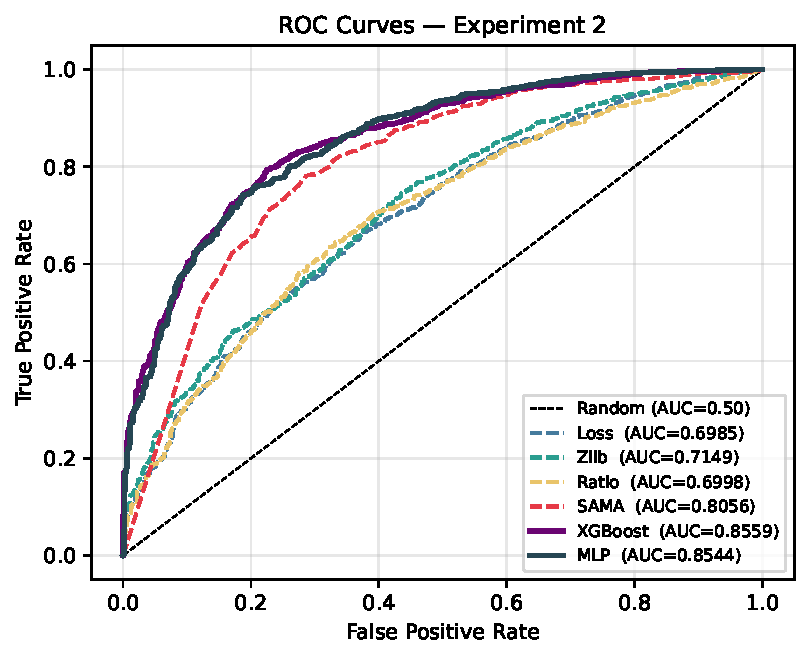
\includegraphics[width=\textwidth]{benchmark_roc.pdf}
    \caption{Full ROC (FPR $\in [0,1]$)}
  \end{subfigure}\hfill
  \begin{subfigure}[b]{0.48\textwidth}
    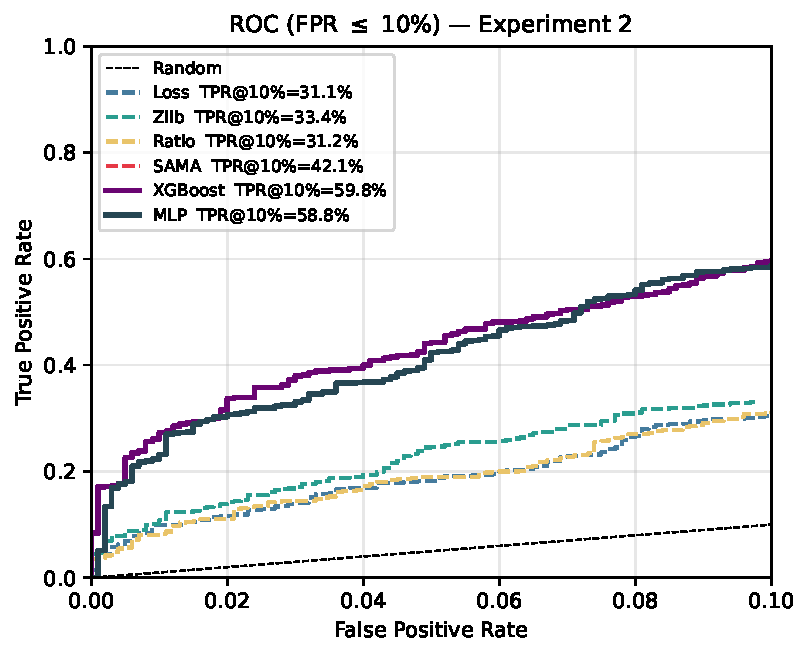
\includegraphics[width=\textwidth]{benchmark_roc_low_fpr.pdf}
    \caption{Zoomed ROC (FPR $\leq 10\%$)}
  \end{subfigure}
  \caption{ROC curves for Experiment 2.  Solid lines: our classifiers.
           Dashed: baselines.  The zoomed panel shows the classifiers
           dominate in the practically relevant low-FPR regime.}
  \label{fig:roc}
\end{figure}

\begin{figure}[h]
  \centering
  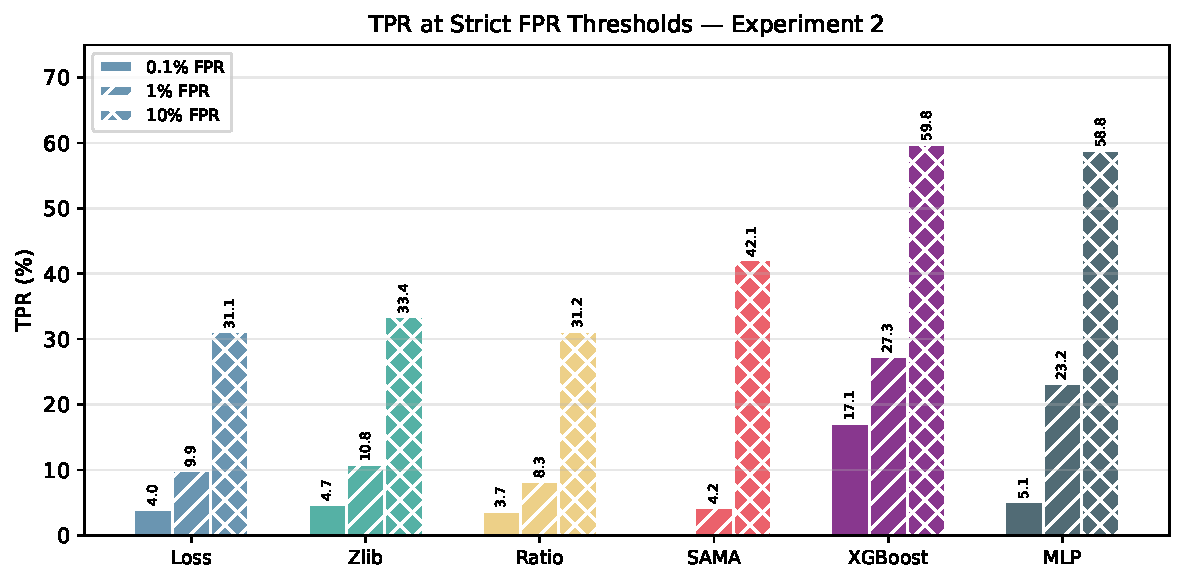
\includegraphics[width=0.88\textwidth]{tpr_all_methods.pdf}
  \caption{TPR (\%) at 0.1\%, 1\%, and 10\% FPR for all methods (Experiment 2).
           XGBoost and MLP (rightmost bars) achieve substantially higher TPR
           at every threshold, with the advantage largest at 0.1\% FPR.}
  \label{fig:tpr}
\end{figure}

% ──────────────────────────────────────────────────────────────────────────────
\section{Future Work}
\label{sec:future}

\paragraph{Complete SAMA-paper benchmark.}
Experiment 2 validates our pipeline on a single MIMIR subset and model.
We will replicate the full evaluation from \citet{shi2025sama}---all nine
MIMIR domain subsets (github, wikipedia, arxiv, pile-cc, dm\_mathematics,
hackernews, pubmed, europarl, enron) plus the additional datasets used in
the SAMA paper---and extend to larger DLMs (e.g.\ LLaDA-8B~\citep{nieLLaDA2025}).

\paragraph{Per-instance privacy auditing (Wei et al.).}
\citet{wei2023pdp} establish that per-instance DP leakage in discrete diffusion
correlates with how \emph{isolated} each training sample is relative to the
distribution.  An open question is whether empirical MIA success rates against
fine-tuned DLMs exhibit the same per-sample structure---and whether attack
scores (e.g.\ our 112-dim features) can serve as practical proxies for the
theoretical $\varepsilon_i$-DP leakage quantities they characterise.

\paragraph{Masking-ratio trajectory as a privacy signal.}
\citet{wei2023pdp} show that leakage concentrates in the low-noise regime.
In masked diffusion, the per-sample loss curve across masking ratios
(already partially captured by our feature vector) may therefore encode
richer privacy information than a scalar NLL.  Investigating the \emph{shape}
of this trajectory---and whether it improves membership classification beyond
our current features---is a natural next step.

\paragraph{Theoretical pDP for absorbing-state DLMs.}
The analysis of \citet{wei2023pdp} is developed for categorical-noise
discrete diffusion; masked diffusion uses a structurally different
absorbing-state forward process (Eq.~\ref{eq:d3pm}).  Whether the
pDP bounds and qualitative leakage insights carry over to the absorbing-state
setting is an open theoretical problem worth pursuing.

\paragraph{Masking-structure-aware private fine-tuning.}
\citet{dockhorn2022dpdm} show that the iterative structure of continuous
diffusion enables a \emph{noise-multiplicity} technique that improves
DP-SGD privacy-utility trade-offs.  The discrete masking structure of MDLM
may admit an analogous exploitation: multiple independent masking realisations
of the same sequence could be used as multiple gradient contributions within a
single DP-SGD step, potentially improving over standard DP-LoRA baselines.

% ──────────────────────────────────────────────────────────────────────────────
\bibliographystyle{plainnat}
\bibliography{refs}

% ──────────────────────────────────────────────────────────────────────────────
\appendix
\section{Additional Figures}

\begin{figure}[h]
  \centering
  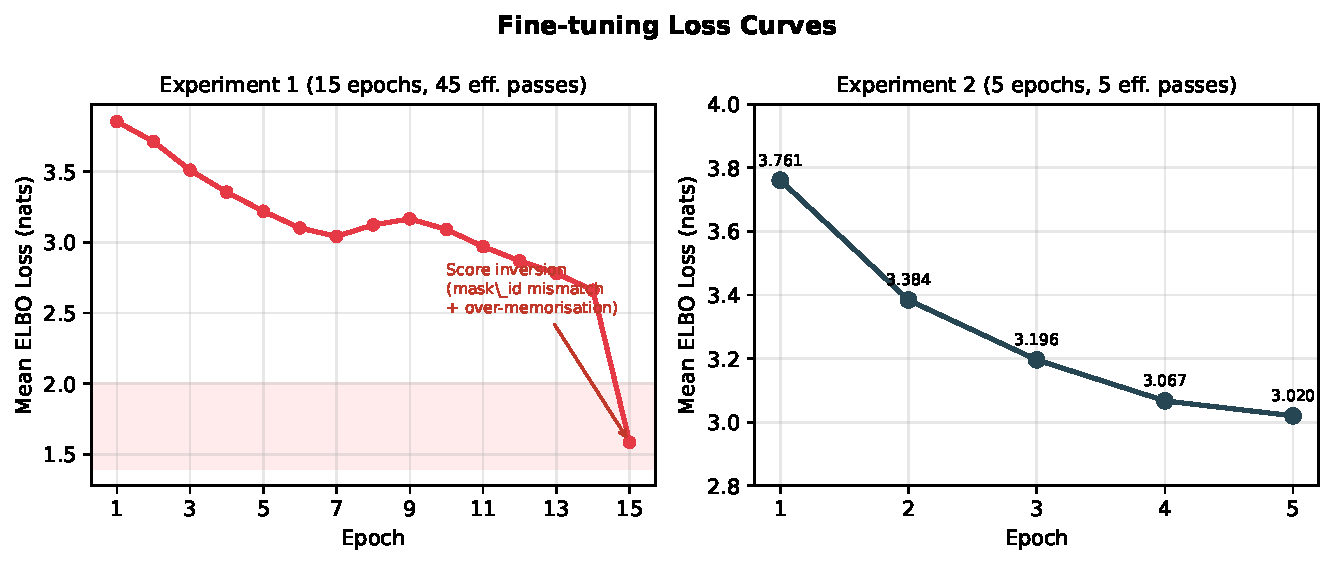
\includegraphics[width=0.92\textwidth]{training_curves.pdf}
  \caption{Fine-tuning loss curves.
           \textbf{Left}: Experiment 1 (15 epochs, 45 effective passes).
           The annotation marks the AUC inversion caused by the mask-token-id
           mismatch (amplified by over-memorisation).
           \textbf{Right}: Experiment 2 (5 epochs); the loss plateaus above
           $3.0$ nats, consistent with moderate---rather than pathological---memorisation.}
  \label{fig:training}
\end{figure}

\begin{figure}[h]
  \centering
  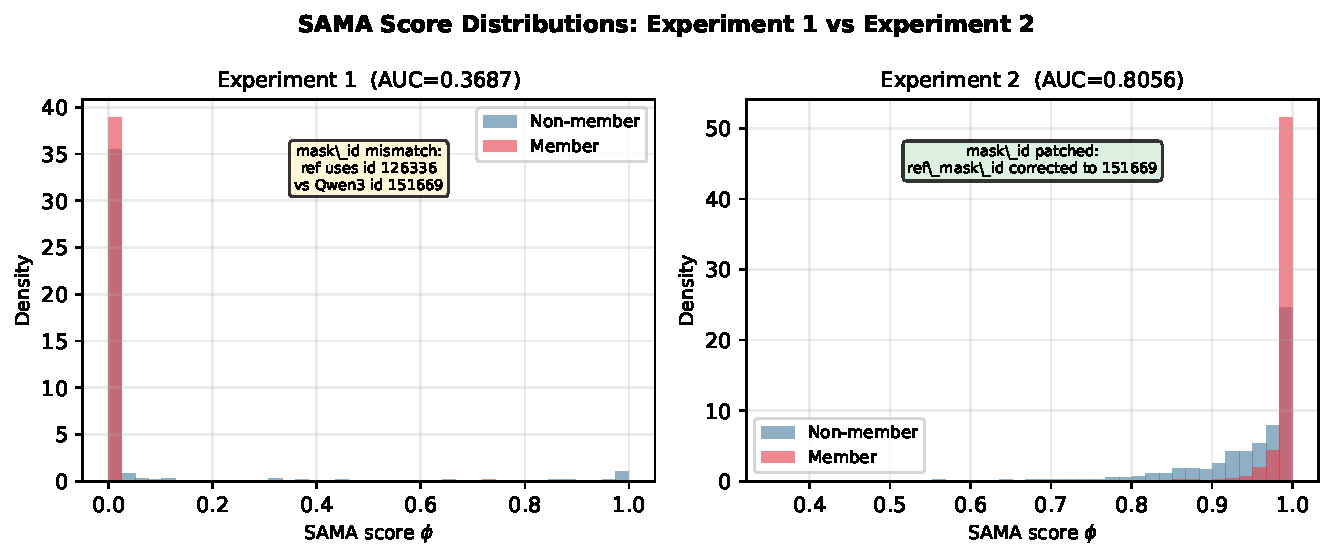
\includegraphics[width=0.92\textwidth]{exp1_vs_exp2_sama.pdf}
  \caption{SAMA score distributions for members (red) and non-members (blue).
           \textbf{Left}: Experiment 1 --- nearly identical distributions with
           slight inversion (AUC\,=\,0.369), caused by the mask-token-id mismatch.
           \textbf{Right}: Experiment 2 --- clear separation (AUC\,=\,0.806)
           after patching \texttt{ref\_mask\_id} to 151\,669.}
  \label{fig:samacomp}
\end{figure}

\begin{figure}[h]
  \centering
  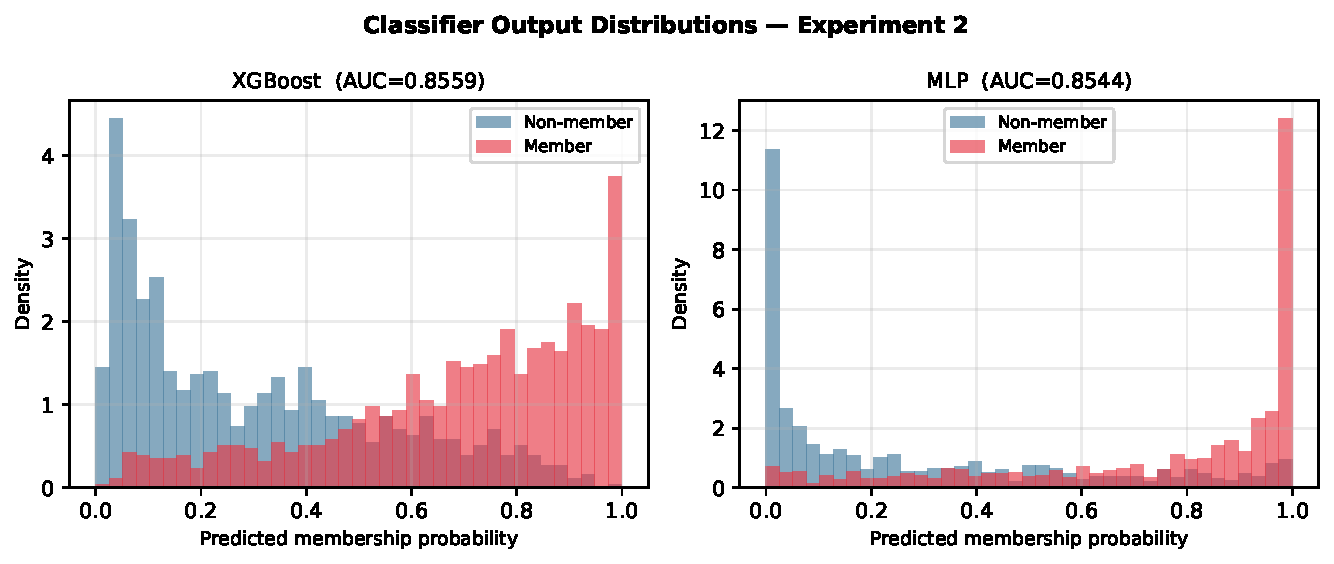
\includegraphics[width=0.90\textwidth]{classifier_score_dist.pdf}
  \caption{Predicted membership probability distributions for XGBoost (left)
           and MLP (right) in Experiment 2.
           Both classifiers separate members (red) from non-members (blue);
           XGBoost shows a sharper peak near 1.0 for members, explaining
           its higher TPR at strict FPR thresholds.}
  \label{fig:clfdist}
\end{figure}

\begin{figure}[h]
  \centering
  
\includegraphics[width=\textwidth]{feature_heatmap.pdf}
  \caption{Mean feature values per class and their signed difference.
           Indices 0--39: ELBO loss at 10 timesteps; 40--79: predictive
           entropy; 80--109: denoising consistency; 110: area-under-loss-curve;
           111: cross-model cosine similarity.
           The strongest discriminative signal concentrates at low noise levels
           (indices 0--9 and 80--89), consistent with \citet{wei2023pdp}'s
           finding that leakage concentrates in the low-noise regime.}
  \label{fig:heatmap}
\end{figure}

\begin{figure}[h]
  \centering
  
\includegraphics[width=0.78\textwidth]{benchmark_bar.pdf}
  \caption{AUC-ROC for all methods.  The grey bar (Experiment 1 SAMA = 0.369)
           is shown as a historical reference, illustrating the mask-token-id
           failure.  Experiment 2 resolves this: SAMA reaches 0.806 and our
           classifiers push further to 0.856.}
  \label{fig:bar}
\end{figure}

\end{document}
